\documentclass[convert={ghostscript,gsdevice=tiffg4,
outext=.tiff,density=1200}]{standalone}
    \usepackage{tikz}
    \usepackage{pgfplots}
    \usetikzlibrary{patterns}
\mathversion{bold}
\begin{document}
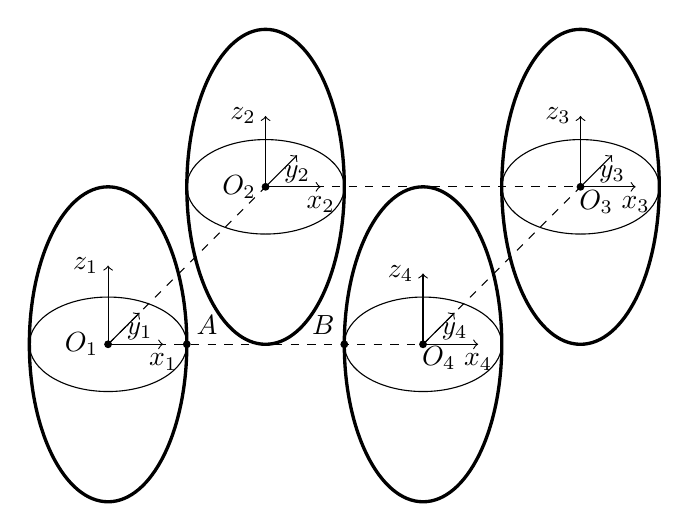
\begin{tikzpicture}%[scale=1.5]
  \draw[->] (0,0) -- (0.7,0) node[anchor=north] {$x_1$};
  \draw[->] (0,0) -- (0,1) node[anchor=east] {$z_1$};
  \draw[->] (0,0) -- (0.4,0.4) node[anchor=north] {$y_1$};
  \draw[->] (4.0,0) -- (4.7,0) node[anchor=north] {$x_4$};
  \draw[->] (4.0,0) -- (4.0,0.9) node[anchor=east] {$z_4$};
  \draw[->] (4.0,0) -- (4.4,0.4) node[anchor=north] {$y_4$};
  \draw[->] (2,2) -- (2.7,2) node[anchor=north] {$x_2$};
  \draw[->] (2,2) -- (2,2.9) node[anchor=east] {$z_2$};
  \draw[->] (2,2) -- (2.4,2.4) node[anchor=north] {$y_2$};
  \draw[->] (6,2) -- (6.7,2) node[anchor=north] {$x_3$};
  \draw[->] (6,2) -- (6,2.9) node[anchor=east] {$z_3$};
  \draw[->] (6,2) -- (6.4,2.4) node[anchor=north] {$y_3$};
%  \draw[->] (2.5,2) -- (6.5,2) node[anchor=north] {$y_2$};
%  \draw[->] (2.5,2) -- (2.5,6) node[anchor=east] {$z_2$};
%  \draw[->] (2.5,2) -- (1.0,-0.5) node[anchor=north] {$x_2$};

\node[left] at (0,0) {$O_1$};
\node[left] at (2.,2) {$O_2$};
\node[below] at (4.2,0.1) {$O_4$};
\node[below] at (6.2,2.08) {$O_3$};
\node[above right] at (1.0,0) {$A$};
\node[above left] at (3,0) {$B$};

%  \node[above] at (1.05,1) {$r_{12}$};
%  \node[above] at (0,-1) {$\varphi_{12}$};
%  \node[right] at (0,1) {$\theta_{12}$};

  \draw[very thick] (0,0) ellipse (1.0 and 2);
  \draw (0,0) ellipse (1.0 and .6);

  \draw[very thick] (4.0,0) ellipse (1.0 and 2);
  \draw (4.0,0) ellipse (1.0 and .6);

  \draw[very thick] (2.,2) ellipse (1.0 and 2);
  \draw (2.,2) ellipse (1.0 and .6);

  \draw[very thick] (6.,2) ellipse (1.0 and 2);
  \draw (6.,2) ellipse (1.0 and .6);

%  \draw (0,0) -- (2.5,2);
%  \draw[dashed] (2.5,2) -- (2.5,-2.5);
%  \draw[dashed] (0,0) -- (2.5,-2.5);

  \node[circle, fill=black, inner sep=1pt] at (0,0) {};
  \node[circle, fill=black, inner sep=1pt] at (2.,2) {};
  \node[circle, fill=black, inner sep=1pt] at (4.0,0) {};
  \node[circle, fill=black, inner sep=1pt] at (6.,2) {};
  \node[circle, fill=black, inner sep=1pt] at (1.0,0) {};
  \node[circle, fill=black, inner sep=1pt] at (3,0) {};
  
  \draw[dashed] (0,0) -- (4.0,0);
  \draw[dashed] (0,0) -- (2.,2);
  \draw[dashed] (2.,2) -- (6.,2);
  \draw[dashed] (4.0,0) -- (6.,2);
\end{tikzpicture}
\end{document}

%%% Local Variables: 
%%% mode: latex
%%% TeX-master: t
%%% End: 
